\documentclass{article}

\usepackage{fancyhdr}
\usepackage{extramarks}
\usepackage{amsmath}
\usepackage{amsthm}
\usepackage{amsfonts}
\usepackage{tikz}
\usepackage[plain]{algorithm}
\usepackage{algpseudocode}
\usepackage{graphicx}
\usepackage{gensymb}
\usepackage[framed,numbered,autolinebreaks,useliterate]{mcode}
\usepackage{listings}

\graphicspath{{./images/}}

\usetikzlibrary{automata,positioning}

%
% Basic Document Settings
%

\topmargin=-0.45in
\evensidemargin=0in
\oddsidemargin=0in
\textwidth=6.5in
\textheight=9.0in
\headsep=0.25in

\linespread{1.1}

\pagestyle{fancy}
\lhead{\hmwkAuthorName}
\chead{\hmwkClass\ \hmwkTitle}
\rhead{\firstxmark}
\lfoot{\lastxmark}
\cfoot{\thepage}

\renewcommand\headrulewidth{0.4pt}
\renewcommand\footrulewidth{0.4pt}

\setlength\parindent{0pt}

%
% Create Problem Sections
%

\newcommand{\enterProblemHeader}[1]{
    \nobreak\extramarks{}{Problem {#1} continued on next page\ldots}\nobreak{}
    \nobreak\extramarks{Problem {#1} (continued)}{Problem {#1} continued on next page\ldots}\nobreak{}
}

\newcommand{\exitProblemHeader}[1]{
    \nobreak\extramarks{Problem {#1} (continued)}{Problem {#1} continued on next page\ldots}\nobreak{}
    % \stepcounter{#1}
    \nobreak\extramarks{Problem {#1}}{}\nobreak{}
}

\setcounter{secnumdepth}{0}
\newcounter{partCounter}

\newcommand{\problemNumber}{0.0}

\newenvironment{homeworkProblem}[1][-1]{
    \renewcommand{\problemNumber}{{#1}}
    \section{Problem \problemNumber}
    \setcounter{partCounter}{1}
    \enterProblemHeader{\problemNumber}
}{
    \exitProblemHeader{\problemNumber}
}

%
% Homework Details
%   - Title
%   - Class
%   - Author
%

\newcommand{\hmwkTitle}{Homework\ \#3}
\newcommand{\hmwkClass}{RBE 500}
\newcommand{\hmwkAuthorName}{\textbf{Arjan Gupta}}

%
% Title Page
%

\title{
    \vspace{2in}
    \textmd{\textbf{\hmwkClass\ \hmwkTitle}}\\
    \vspace{3in}
}

\author{\hmwkAuthorName}
\date{}

\renewcommand{\part}[1]{\textbf{\large Part \Alph{partCounter}}\stepcounter{partCounter}\\}

%
% Various Helper Commands
%

% Useful for algorithms
\newcommand{\alg}[1]{\textsc{\bfseries \footnotesize #1}}

% For derivatives
\newcommand{\deriv}[1]{\frac{\mathrm{d}}{\mathrm{d}x} (#1)}

% For partial derivatives
\newcommand{\pderiv}[2]{\frac{\partial}{\partial #1} (#2)}

% Integral dx
\newcommand{\dx}{\mathrm{d}x}

% Alias for the Solution section header
\newcommand{\solution}{\textbf{\large Solution}}

% Probability commands: Expectation, Variance, Covariance, Bias
\newcommand{\E}{\mathrm{E}}
\newcommand{\Var}{\mathrm{Var}}
\newcommand{\Cov}{\mathrm{Cov}}
\newcommand{\Bias}{\mathrm{Bias}}

\begin{document}

\maketitle

\nobreak\extramarks{Problem 4.2}{}\nobreak{}

\pagebreak

\begin{homeworkProblem}[4.2]
    Verify Equation (4.7) by direct calculation.

    \[
        S(a)p = a \times p \tag{4.7}
    \]

    \subsection{Solution}

    Suppose the vectors $a$ and $p$ are given as

    \[
        a =
            \begin{bmatrix}
                a_1\\
                a_2\\
                a_3
            \end{bmatrix},
        p =
            \begin{bmatrix}
                p_1\\
                p_2\\
                p_3
            \end{bmatrix}
    \]

    By the definition of the cross-product, we know
    \begin{align}
        a \times p =
        \begin{bmatrix}
            a_2p_3 - a_3p_2\\
            a_3p_1 - a_1p_3\\
            a_1p_2 - a_2p_1
        \end{bmatrix}
    \end{align}

    Also, by the definition of skew-symmetric matrices, we know the form of $S(a)$, where $a$ is the vector we have already defined,
    \[
        S(a) =
        \begin{bmatrix}
            0 & -a_z & a_y\\
            a_z & 0 & -a_x\\
            -a_y & a_x & 0\\
        \end{bmatrix}
    \]
    Hence, by normal matrix multiplication,
    \[
        S(a) p =
        \begin{bmatrix}
            0 - a_3p_2 + a_2p_3\\
            a_3p_1 + 0 -a_1p_3\\
            -a_2p_1 + a_1p_2 + 0
        \end{bmatrix}
        =
        \begin{bmatrix}
            a_2p_3 - a_3p_2\\
            a_3p_1 - a_1p_3\\
            a_1p_2 - a_2p_1
        \end{bmatrix}
    \]

    Which is the same as (1). Therefore, Equation (4.7) is proved.
\end{homeworkProblem}

\nobreak\extramarks{Problem 4.3}{}\nobreak{}

\pagebreak

\newcommand\norm[1]{\lVert#1\rVert}

\begin{homeworkProblem}[4.3]
    Prove the assertion given in Equation (4.9) that \(R (a \times b) = Ra \times Rb \) for \(R \in SO(3)\).

    \vspace{0.1in}
    \subsection{Solution}
    Let \(v = R (a \times b)\), and \(u = Ra \times Rb \). If $v$ and $u$ are the to be proved as the same vector, then
    it must be shown that they have the exact same magnitude and direction. Let us consider magnitude and direction of
    $v$ and $u$ separately.

    \subsubsection{Magnitude}

    Since \(R \in SO(3)\), \(\det{R} = 1\), which means that the linear transformation $R$ does not change the length (norm) of
    any vector that it transforms (rotates). Hence we can say

    \begin{align}        
        \norm{R(a \times b)} &= \norm{a \times b} \tag{1}\\
        \norm{Ra} &= \norm{a}\\
        \norm{Rb} &= \norm{b}
    \end{align}

    Using the definition of the cross product along with (1), we can state that
    \begin{align}
        \norm{v} = \norm{R(a \times b)} = \norm{a \times b} = \norm{a}\norm{b}\sin\theta
    \end{align}
    
    Again using the definition of the cross product along with (2) and (3), we can state that 
    \begin{align}
        \norm{u} = \norm{Ra \times Rb} = \norm{Ra}\norm{Rb}\sin\theta = \norm{a}\norm{b}\sin\theta
    \end{align}

    We can see that (4) and (5) are equal. Therefore,
    \[
        \norm{v} = \norm{u}
    \]
    Which means that the magnitude of $v$ and $u$ are the same.

    \subsubsection{Direction}

    Since \(R \in SO(3)\) is a merely a rotational transformation of the 3 dimensional vector space, any directional relationships given
    by the right-hand curl rule before $R$ has been applied must remain preserved and obtainable by the right-hand curl rule even after $R$
    has been applied.
    \vspace{0.15in}

    Now, let us assume that the vectors $a$ and $b$ lie in the plane $P$. Also, assume \(a \times b\) lies in the direction gvien by
    $\hat{q}$. We know that $\hat{q}$ can be obtained by applying the right-hand curl rule from $a$ to $b$.
    \vspace{0.15in}
    
    After $R$ is applied, $P$ becomes plane $P_R$, and $\hat{q}$ becomes $\hat{q_R}$. This means that \(v = R (a \times b)\) 
    lies along $\hat{q_R}$. Also, vector $a$ and $b$ become vectors $Ra$ and $Rb$, which now lie in plane $P_R$.
    However, we can still obtain $\hat{q_R}$ by applying the right-hand curl rule from $Ra$ to $Rb$, since this relationship is preserved.
    Hence, \(u = Ra \times Rb \) lies in the direction $\hat{q_R}$. Therefore, $v$ and $u$ lie in the same direction.
    \vspace{0.15in}

    Since $v$ and $u$ lie in the same direction and have the same magnitude, they are the same vector. Hence, (4.9) is proved.
\end{homeworkProblem}

\nobreak\extramarks{Problem 4.5}{}\nobreak{}

\pagebreak

\begin{homeworkProblem}[4.5]
    Suppose that $a$ = (1,-1,2) and that \(R = R_{x,90}\). Show by direct calculation that \(RS(a)R^T = S(Ra)\).

    \subsection{Solution}

    \begin{align*}
        R = R_{x,90}
        &= \begin{bmatrix}
            1 & 0 & 0\\
            0 & \cos(90) & -\sin(90)\\
            0 & \sin(90) & \cos(90)
        \end{bmatrix}
        = \begin{bmatrix}
            1 & 0 & 0\\
            0 & 0 & -1\\
            0 & 1 & 0
        \end{bmatrix}\\\\    
        S(a) &=  \begin{bmatrix}
            0 & -2 & -1\\
            2 & 0 & -1\\
            1 & 1 & 0
        \end{bmatrix}\\\\
        RS(a)R^T &=
        % Step 1
        \left(\begin{bmatrix}
            1 & 0 & 0\\
            0 & 0 & -1\\
            0 & 1 & 0
        \end{bmatrix}
        \begin{bmatrix}
            0 & -2 & -1\\
            2 & 0 & -1\\
            1 & 1 & 0
        \end{bmatrix}\right)
        \begin{bmatrix}
            1 & 0 & 0\\
            0 & 0 & 1\\
            0 & -1 & 0
        \end{bmatrix}\\
        &= 
        % Step 2
        \begin{bmatrix}
            0 & -2 & -1\\
            -1 & -1 & 0\\
            2 & 0 & -1
        \end{bmatrix}
        \begin{bmatrix}
            1 & 0 & 0\\
            0 & 0 & 1\\
            0 & -1 & 0
        \end{bmatrix}\\
        &=
        % Step 3
        \begin{bmatrix}
            0 & 1 & -2\\
            -1 & 0 & -1\\
            2 & 1 & 0
        \end{bmatrix}\\
        \\
        % RHS side computations
        Ra &= \begin{bmatrix}
            1 & 0 & 0\\
            0 & 0 & -1\\
            0 & 1 & 0
        \end{bmatrix}
        \begin{bmatrix}
            1\\
            -1\\
            2
        \end{bmatrix}
        = \begin{bmatrix}
            1\\
            -2\\
            -1
        \end{bmatrix}\\
        S(Ra) &=
        \begin{bmatrix}
            0 & 1 & -2\\
            -1 & 0 & -1\\
            2 & 1 & 0
        \end{bmatrix}
    \end{align*}
    As we can see, it has been shown that \(RS(a)R^T = S(Ra)\).
\end{homeworkProblem}

\nobreak\extramarks{ROS Report}{}\nobreak{}

\pagebreak

\section{Jacobian Problem}

Derive the Jacobian for the following image.

\begin{figure}[h]
    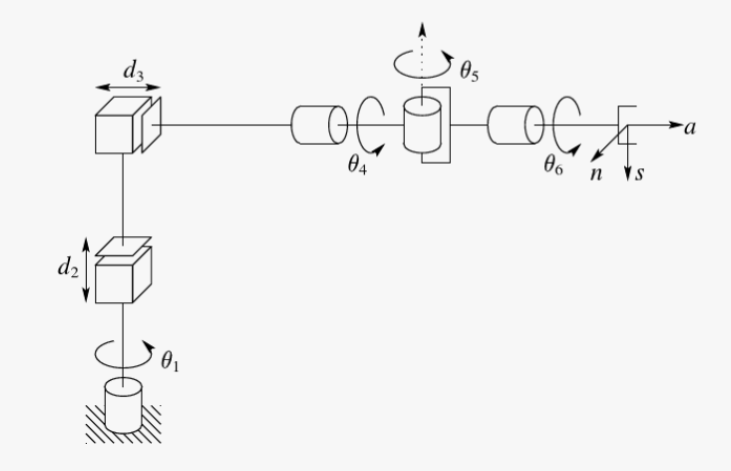
\includegraphics[scale=0.25]{jacobian-prob.png}
    \centering
\end{figure}

\subsection{Solution}

For easy visualization, let us draw the z axes for each joint.
\begin{figure}[h]
    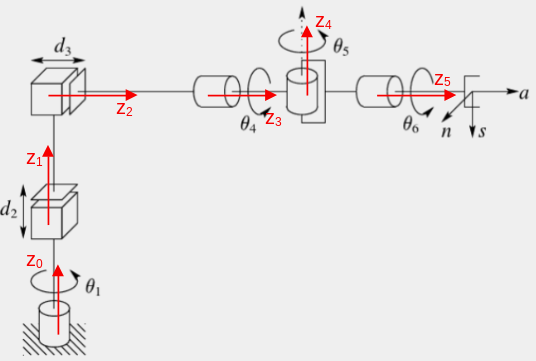
\includegraphics[scale=0.5]{jacobian-prob-sketched.png}
    \centering
\end{figure}

We can see that we have 6 joints, so $n = 6$. Let us also form the table given in the lecture videos:

\begin{table}[h!]
    \begin{center}
        \begin{tabular}{|c|c|c|}
        \hline
        & Linear component & Angular component\\
        \hline
        Revolute joint & \(J_{v_i} = z^0_{i-1} \times (o^0_n - o^0_{i-1})\) & \(J_{v_i} = z^0_{i-1}\) \\
        Prismatic joint & \(J_{\omega_i} = z^0_{i-1}\) & \(J_{\omega_i} = 0\)\\
        \hline
        \end{tabular}
    \end{center}
\end{table}

Using this table, and the fact that the upper half of the Jacobian contains linear components while the bottom half
contains angular components, we have
\[
    J =
    \begin{bmatrix}
        z_{0} \times (o_6 - o_{0}) & z_1 & z_2 & z_3 \times (o_6 - o_3) & z_4 \times (o_6 - o_4) & z_5 \times (o_6 - o_5) \\
        z_0 & 0 & 0 & z_3 & z_4 & z_5
    \end{bmatrix}
\]

\pagebreak

\section{Report for ROS2 Portion}

For this week's ROS assignment portion, I created a subscriber just like how
we did for last week's assignment. I also used the same ros2 command type as
the one last week, specifically,
\lstinline{ros2 topic pub --once <topic_name> <data_type> <data>}.
\vspace{0.17in}
\\Futhermore, this week I set up my subscriber to accept 3 joint variable 
values from the publisher. These 3 values are floats that represent the
angles for the three revolute joints (\(\theta_1, \theta_2, \theta_3\))
of the robot manipulator we considered in Problem 3.5 of Homework \#2. Using
\(\theta_1, \theta_2, \theta_3\), my subscriber calculated forward kinematics
using the symbolic T matrix I calculated last week, given by
\[
    T_3^0 =
    \begin{bmatrix}
        c_{1}\,c_{2}\,c_{3}-c_{1}\,s_{2}\,s_{3} & -c_{1}\,c_{2}\,s_{3}-c_{1}\,c_{3}\,s_{2} & -s_{1} & a_{2}\,c_{1}\,c_{2}-a_{3}\,c_{1}\,s_{2}\,s_{3}+a_{3}\,c_{1}\,c_{2}\,c_{3}\\
        c_{2}\,c_{3}\,s_{1}-s_{1}\,s_{2}\,s_{3} & -c_{2}\,s_{1}\,s_{3}-c_{3}\,s_{1}\,s_{2} & c_{1} & a_{2}\,c_{2}\,s_{1}-a_{3}\,s_{1}\,s_{2}\,s_{3}+a_{3}\,c_{2}\,c_{3}\,s_{1}\\
        -c_{2}\,s_{3}-c_{3}\,s_{2} & s_{2}\,s_{3}-c_{2}\,c_{3} & 0 & d_{1}-a_{2}\,s_{2}-a_{3}\,c_{2}\,s_{3}-a_{3}\,c_{3}\,s_{2}\\
        0 & 0 & 0 & 1
    \end{bmatrix}
\]
I imported the \lstinline{numpy} python package to put this $T_3^0$ matrix in a
\lstinline{numpy.array}, and then I printed the matrix for the given joint variables.
In my code, I made sure to name $c_i$ and $s_i$ exactly that way so that I could
visually verify any issues in setting up the matrix. The \lstinline{math.cos} and
\lstinline{math.sin} python functions were used to for assigning values to $c_i$
and $s_i$. I also set $d_1, a_2, a_3$ as 1 to make sure I could easily verify
that my code is working correctly.
\end{document}